\section{A Reporting Design and its Evaluation}
\label{sec:design}

Secs.~\ref{sec:outages}--\ref{sec:reconstruct} point to a design: buffer and back off through gaps (only delivery restores long gaps), batch routine data (cheap, and little less timely when gaps are long), and show the site's own diel estimate between deliveries. Batching leaves two gaps, alarms and the real-time picture of fast parameters, and the design closes them with two triggers that send a batch early.

\subsection{The design}
\label{sec:des-design}
\emph{Event-driven batching} runs at the node (Algorithm~\ref{alg:design}, without the bounded-error trigger). Every reading is buffered. Once an hour the node uploads its buffer in confirmed bulk frames. When the node's event detector raises an alarm, it uploads the buffer at once, alarming reading included; if the node is in an outage, an alarm triggers an immediate probe outside the back-off schedule (without resetting it). A failed upload puts the node into outage mode, with the probe back-off (\ref{eq:backoff}).

Fig.~\ref{fig:mechanism} shows these behaviours in a short illustrative scenario run through the simulator. Before the outage, the alarm makes the event-driven node upload at once, where plain batching would wait for the end of the hour; the alarm during the outage cannot get through; and after the outage, when the backlog arrives depends on where each strategy is in its back-off (\ref{eq:backoff}).

\begin{figure*}[t]
\centering
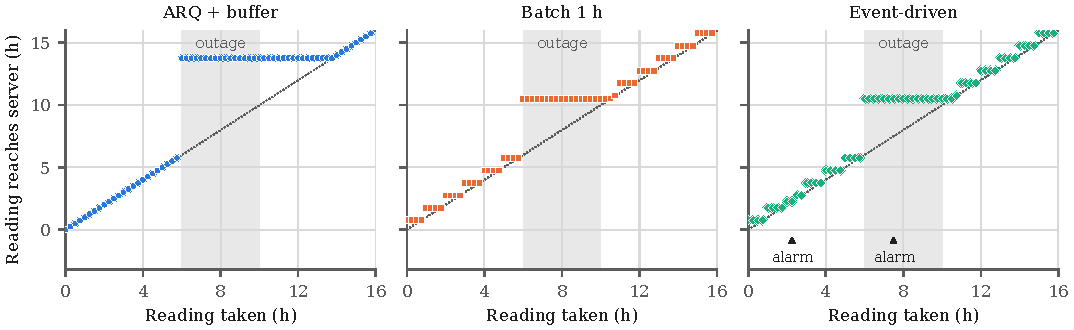
\includegraphics[width=\textwidth]{fig_mechanism}
\caption{When each reading reaches the server, in an illustrative scenario run through the simulator: LoRaWAN SF7, 15-min sampling, the link down from 6 to 10~h, and node alarms at 2.25~h (link up) and 7.5~h (link down). Points on the dotted diagonal arrive at once; horizontal runs are readings delivered together. Event-driven batching follows hourly batching except that the alarm at 2.25~h sends its batch early.}
\label{fig:mechanism}
\end{figure*}

\emph{Bounded event-driven batching} adds a \emph{bounded-error trigger}. Because every upload is confirmed, the node knows which of its readings have reached the server and when; it can therefore compute, at every slot $t$, the value $\hat{x}_j(t)$ that the server is showing for each parameter $j$, by evaluating (\ref{eq:picture}) on the readings it knows to have arrived. It uploads its buffer at once (Algorithm~\ref{alg:design}) if
\begin{equation}
\max_{j}\ \frac{|x_j(t)-\hat{x}_j(t)|}{\delta_j}>1,
\label{eq:trigger}
\end{equation}
that is, if any parameter's true reading differs from what the server shows by more than its tolerance $\delta_j$. This is the dual-prediction mechanism of error-bounded report suppression~\cite{dias2016survey,santini2006adaptive}, used here to bound the error between batches rather than to suppress reports. Three details matter. First, the trigger is not consulted during an outage: the server's estimate may drift far from the truth during a long gap, and a node that probed every time would waste energy on a dead link; only alarms probe. Second, the node's copy of the server must model \emph{when} readings arrive, not only \emph{whether}: on LoRaWAN the duty cycle spaces the frames of a long upload, so a reading enters $A(t)$ in (\ref{eq:picture}) only after its frame's arrival time, and the newest valid reading goes in the first frame of every upload, so that the value the server most needs arrives first. Third, the node's knowledge of the server comes from acknowledgements, so it is only as good as their boundary. On NB-IoT the confirmation is the application server's reply~\cite{michelinakis2021dissecting}, and the node knows what the server holds. On LoRaWAN a confirmed uplink is acknowledged by the network server; the forwarding to the application server, which UVA's ``system'' losses show can fail, is not covered. A variant of the trigger closes this gap at a cost (Sec.~\ref{sec:des-ack}): it keeps the bound for both possible server states, with and without the readings the network server acknowledged, until an application acknowledgement returns in the downlink of a later uplink.

\begin{algorithm}[t]
\caption{Bounded event-driven batching: node, one slot}
\label{alg:design}
\small
\begin{algorithmic}[1]
\State append the slot's reading $x_t$ to the buffer
\If{in outage mode}
  \If{alarm at $t$ \textbf{or} back-off timer expired} \State probe; on success leave outage mode and upload the buffer \EndIf
  \State \Return
\EndIf
\State $\hat{x}(t) \gets$ server's estimate (\ref{eq:picture}), from readings whose arrival time is $\le t$
\If{alarm at $t$ \textbf{or} trigger (\ref{eq:trigger}) \textbf{or} hour boundary}
  \State upload the buffer (newest valid reading first), confirmed bulk frames
  \State on failure enter outage mode, back-off (\ref{eq:backoff})
\EndIf
\end{algorithmic}
\end{algorithm}

\subsection{Evaluation protocol}
\label{sec:des-protocol}
\emph{Two phases.} The design was developed on 2023 data and then tested on held-out 2024 data. In the development phase, hypotheses H1--H4 and their decision rules were written down before the runs for event-driven batching; after H4 failed, H5--H7 were written for the bounded-error trigger before it was implemented, and H8--H10, on packing order and on the tolerance level, before they were run. Every deviation was recorded when made, with its reason: UVA replayed as system outages plus radio losses (D1); one site excluded because its eligibility had been computed over its record span rather than the year (D2); seeds derived from site identifiers (D3); two implementation defects of the packing order, which made H8 fail as written (D4); and a floating-point tie at the tolerance (D5, found during the revision): pH and T are recorded in 0.1 steps, and an error of exactly one tolerance was counted in or out by rounding noise, in the scores and in the trigger. All development results below are from a rerun with D4 and D5 fixed. For the confirmatory phase, the final design, the analysis code, its decision rules and the eligibility rule were frozen, and the code identified by cryptographic hashes, before any 2024 data were downloaded; the 2024 verdicts below are the output of that frozen code. The plans are kept with the code and hashed; they were not registered with a third party.

\emph{Sites.} Every USGS site of the \designCandidates{} candidates with all four parameters in complete cycles for at least half of the year: \designSites{} sites in 2023 and \confSites{} in 2024 (\sitesBothYears{} in both years). Sampling steps are 5 to 60~min. The first 20\% of each record trains the detector; all metrics are computed on the remaining 80\%.

\emph{Links.} The no-outage link, and three real records mapped onto each site's time grid in physical time, wrapped circularly with a random start offset per site (seeded by the site identifier, with a different seed in 2024): InWaterSense and Weija conductivity, in which every missing slot is a down link (the full-slot model, pessimistic for the per-reading strategies), and UVA, replayed as its system outages plus independent radio losses at the rate of a representative sensor (\uvaSensorFourRadio{} per attempt). \emph{Radios:} NB-IoT ($T_\mathrm{search}=10$~s), LoRaWAN SF7 and SF12.

\emph{Strategies.} Unconfirmed, ARQ + buffer, hourly batching (``batch 1~h''), event-driven batching, and bounded event-driven batching (newest-first packing, L2 tolerance unless stated), as defined above and in Sec.~\ref{sec:data-energy}.

\emph{Injected events.} Events are added to the real test-period series, so background dynamics, noise and gaps are real and only the event is synthetic. For parameter $j$, let $a_j(t)$ be the reading minus its centred 24-h running median, and $r_j(t)$ that anomaly minus its median for the same calendar month and hour of day. The event scale is the robust standard deviation of $r_j$ in the event's month,
\begin{equation}
\sigma_j=\max\left(1.4826\,\operatorname{MAD}\!\left[r_j\right],\ \rho_j\right),
\label{eq:scale}
\end{equation}
floored at the recording resolution $\rho_j$, estimated from the data as the most common positive difference between sorted distinct values. An event of amplitude $\kappa\sigma_j$, with $\sigma_j$ from (\ref{eq:scale}), $\kappa\in\{5,8\}$ and a random sign, lasts 180~min: a \emph{step} adds $\kappa\sigma_j$ for its whole duration, and a \emph{ramp} rises linearly from 0 to $\kappa\sigma_j$; injected values are rounded to $\rho_j$. Events touch one parameter each, in turn, lie in the test period, at least a day after the start of a data segment and wholly inside it, and at least three days apart (at most 60 per site and setting; \designEventsConf{} in 2024). The events are of a realistic size. Their median amplitudes are mild in physical units (5$\sigma$/8$\sigma$: T \ampFiveT/\ampEightT~$^\circ$C, DO \ampFiveDO/\ampEightDO~\%sat, EC \ampFiveEC/\ampEightEC~$\mu$S/cm, pH \ampFivePh/\ampEightPh), and real 3-hour changes of at least 5$\sigma$ occur at \realFiveT{} of the sites for T, \realFiveDO{} for DO, \realFiveEC{} for EC and \realFivePh{} for pH (8$\sigma$: \realEightT, \realEightDO, \realEightEC, \realEightPh). They are physically plausible: \plausibleConf{} of the 2024 events stay within T $-0.5$--40~$^\circ$C, positive EC, pH 4--11 and DO 0--250~\%sat (\plausibleDev{} in 2023).

\emph{Detector.} All strategies use the same causal detector: on the node for the event-driven designs, and on the server, on the readings it has received, for the others. It compares each reading with the reading $m=120$~min earlier, corrected by a learned hour-of-day profile $p(\cdot)$ of the departure from the running 24-h median, and runs a two-sided CUSUM~\cite{page1954continuous} on the clipped, standardised residual:
\begin{align}
z_t&=\operatorname{clip}\!\left(\frac{x_t-x_{t-m}-p(h_t)+p(h_{t-m})}{s},\,-c,\,c\right),\label{eq:z}\\
S^{+}_t&=\max\left(0,\,S^{+}_{t-1}+z_t-k\right),\nonumber\\
S^{-}_t&=\max\left(0,\,S^{-}_{t-1}-z_t-k\right),\label{eq:cusum}
\end{align}
where $h_t$ is the hour of day and $s$ a robust residual scale floored at $\rho_j$. An alarm is raised when either sum in (\ref{eq:cusum}), driven by the residual (\ref{eq:z}), exceeds $H$, with $k=3$, $H=8$ and $c=6$; the detector then stays in an event state until $|z_t|<2$ for 60~min, and resets its sums. The profile and the scale are initialised on the training period and updated by exponential smoothing (memory about 7~days) only outside the event state. These parameters were fixed before any evaluation and were not tuned on its data. An event counts as detected if an alarm on its parameter occurs during it. In 2024 the detector caught a median (over sites) of \detectStepFive{} of 5$\sigma$ steps, \detectStepEight{} of 8$\sigma$ steps, \detectRampFive{} of 5$\sigma$ ramps and \detectRampEight{} of 8$\sigma$ ramps (\detectAll{} of all events), with a median of \faMedian{} false alarms per parameter per 30 days (mean \faMean).

\emph{Metrics.} \emph{Alarm latency}: the time from an event's onset to the arrival of its alarm at the server, for detected events, split by whether the link was up at onset. Because an operator cares about the whole chain, the share of \emph{all} injected events that the server knows of within 1, 6 and 24~h is also reported. \emph{Energy}: transmission J/day, $E_\mathrm{tx}$ in (\ref{eq:energy}), including uploads caused by alarms and false alarms; for the event-driven designs, averaged over the four event settings. \emph{Picture}: the share of scored slots at which the server's real-time picture (\ref{eq:picture}) is within tolerance, on the series without injected events. Each is summarised as the median over sites per link and radio (12 link--radio combinations; 48 with the four parameters), with 95\% confidence intervals from resampling sites (10{,}000 draws).

Table~\ref{tab:hyp} lists the hypotheses and their verdicts in both phases.

\begin{table*}[t]
\centering
\caption{Hypotheses, decision rules and verdicts. Each rule applies to the median site of every link--radio combination (12), or of every link--radio--parameter combination (48), and passes only if it holds in all. Phase of writing: P, before the development runs; A, after H4 failed, before the runs concerned. Development: 2023 rerun with D4 and D5 fixed; held-out: 2024, judged by the frozen code. ``Event'' = event-driven batching; ``Bounded'' = bounded event-driven batching.}
\label{tab:hyp}
\small
\begin{tabular}{@{}llp{5.0cm}p{4.6cm}ll@{}}
\toprule
 & & Claim & Rule & 2023 (development) & 2024 (held-out) \\
\midrule
H1 & P & Link up: Event raises alarms as fast as per-reading reporting & Event $-$ ARQ+buffer alarm latency $\le$ 1 slot & Pass, \chOneDev & Pass, \chOneConf \\
H2 & P & Event costs about as much as batching, much less than per-reading ARQ & Event / batch $\le 1.10$ and ARQ+buffer / Event $\ge 1.3$ & Pass, \chTwoDev & Pass, \chTwoConf \\
H3 & P & Onset in an outage: buffering delivers late, unconfirmed loses & descriptive & As expected & As expected \\
H4 & P & Event's picture is as good as per-reading reporting's & Event $\ge$ ARQ+buffer $-$ 5 pp & Fail, \chFourDev & Fail, \chFourConf \\
H5 & A & Bounded's picture is as good as per-reading reporting's & Bounded $\ge$ ARQ+buffer $-$ 1 pp & Pass, \chFiveDev & Pass, \chFiveConf \\
H6 & A & Bounded costs no more than per-reading ARQ & Bounded $\le$ ARQ+buffer energy & Pass, \chSixDev & Pass, \chSixConf \\
H7 & A & The trigger does not delay alarms & Bounded $-$ Event alarm latency $\le$ 1 slot & Pass, \chSevenDev & Pass, \chSevenConf \\
H8 & A & Newest-first packing makes the picture exact with the link up & 100\% within tolerance, no outage, every site & Fail as written; pass after D4 & Pass \\
H9 & A & H5 holds at tolerances L1 and L3 & as H5 & Pass, \chNineLOneDev, \chNineLThreeDev & Pass, \chNineLOneConf, \chNineLThreeConf \\
H10 & A & H6 holds at tolerances L1 and L3 & as H6 & Pass, \chTenLOneDev, \chTenLThreeDev & Pass, \chTenLOneConf, \chTenLThreeConf \\
\bottomrule
\end{tabular}
\end{table*}

\subsection{Alarms with the link up (H1, H7)}
\label{sec:des-alarms}
With the link up at an event's onset, event-driven batching raises alarms at the server as fast as per-reading ARQ in both years (H1; Table~\ref{tab:design}). The median latency of about an hour is the detector's own: the CUSUM needs about an hour of evidence, and delivery adds nothing. Plain hourly batching is slower in every combination, by a median of \batchLagMinConf--\batchLagMaxConf~h in 2024. On the InWaterSense link the event-driven design is never slower than ARQ + buffer, and faster at SF12 in 2024 (on every radio in 2023), because an alarm probes at once while ARQ + buffer waits for its back-off schedule when a gap starts during the event. The bounded-error trigger does not delay alarms (H7). Counting all injected events, detected or not, the server knows of \knownOneEventNoneConf{} within an hour with event-driven batching on the no-outage link at SF7, the same as with per-reading reporting, against \knownOneBatchNoneConf{} with hourly batching; within a day it knows of \knownDayEventNoneConf{} with any of them. On the InWaterSense link the shares within an hour are \knownOneBoundedInwsConf{} (bounded), \knownOneArqInwsConf{} (ARQ + buffer), \knownOneUnconfInwsConf{} (unconfirmed) and \knownOneBatchInwsConf{} (batch), and within a day \knownDayBoundedInwsConf, \knownDayArqInwsConf, \knownDayUnconfInwsConf{} and \knownDayBatchInwsConf. The ceiling is the detector's \detectAll{} detection, not the reporting scheme.

\begin{table}[t]
\centering
\caption{Held-out year (2024): alarm latency with the link up (median over sites of each site's median, hours) and transmission energy (median over sites, J/day); LoRaWAN SF7. Energies of the event-driven designs are averaged over the four event settings. ARQ: ARQ + buffer.}
\label{tab:design}
\scriptsize
\setlength{\tabcolsep}{2.2pt}
\begin{tabular}{@{}lrrrrrrrr@{}}
\toprule
 & \multicolumn{4}{c}{Alarm latency (h)} & \multicolumn{4}{c}{Energy (J/day)} \\
\cmidrule(lr){2-5}\cmidrule(l){6-9}
Link & ARQ & Batch & Event & Bounded & ARQ & Batch & Event & Bounded \\
\midrule
\tabin{tables/tab_design.tex}
\bottomrule
\end{tabular}
\end{table}

\subsection{Energy (H2, H6)}
\label{sec:des-energy}
Alarm uploads are rare (a median of \alarmsPerDay{} alarms per node per day in 2024; mean \alarmsPerDayMean), and most ride on readings that would have been sent within the hour anyway. Event-driven batching therefore costs \eventOverBatchMinConf--\eventOverBatchMaxConf{} as much as plain batching, and ARQ + buffer costs \arqOverEventMinConf--\arqOverEventMaxConf{} as much as event-driven batching (H2). The bounded-error trigger costs more, \boundedOverBatchMinConf--\boundedOverBatchMaxConf{} the energy of plain batching, because each trigger sends an extra upload between batches. Per-reading ARQ still uses \arqOverBoundedMinConf--\arqOverBoundedMaxConf{} as much energy as the bounded design (H6; every site-resampled 95\% interval lies above \arqOverBoundedCiLowConf), against \arqOverBoundedMinDev--\arqOverBoundedMaxDev{} in the development year. At an hourly cadence an hourly batch holds a single reading, so batching cannot save energy there.

\subsection{The real-time picture (H4, H5)}
\label{sec:des-picture}
Table~\ref{tab:picture} and Fig.~\ref{fig:tradeoff} show the server's picture. Plain event-driven batching fails H4 in both years: for DO, an estimate up to an hour old leaves the L2 tolerance between batches, and the picture is \hFourFailMinConf{} to \hFourFailMaxConf{} percentage points less often within tolerance than with per-reading reporting (2023: \hFourFailMinDev{} to \hFourFailMaxDev). The failures occur with no outage at all, so they are a property of hourly batching, not of the gaps. The event detector does not help: these excursions are ordinary diel motion, not events. (In the first development run, H4 also failed for pH, \hFourPassVOne{} combinations passing; the pH failures were the rounding tie D5, not batching.)

The bounded-error trigger removes the failure. The bounded design's picture is within \hFiveDiffMinConf{} to \hFiveDiffMaxConf{} percentage points of per-reading reporting's for every parameter, link and radio (H5; 2023: \hFiveDiffMinDev{} to \hFiveDiffMaxDev). With the link up and no radio loss it is within tolerance at every scored slot, by construction (H8 below).

Under the two water-quality gap records, unconfirmed reporting shows a \emph{better} picture than ARQ + buffer for every parameter and radio (e.g., DO on InWaterSense at SF7: \picInwsDoUnconf{} vs \picInwsDoArq). When the link returns, an unconfirmed node delivers its next reading at once, while a buffering node waits for its next back-off probe. The back-off saves energy and costs timeliness right after gaps; unconfirmed reporting, of course, never delivers the readings lost in them.

\begin{table}[t]
\centering
\caption{Held-out year (2024): share of scored slots within the L2 tolerance (median over sites; LoRaWAN SF7; series without injected events). ARQ: ARQ + buffer.}
\label{tab:picture}
\scriptsize
\setlength{\tabcolsep}{3pt}
\begin{tabular}{@{}llrrrrr@{}}
\toprule
Link & Param. & Unconf. & ARQ & Batch & Event & Bounded \\
\midrule
\tabin{tables/tab_picture.tex}
\bottomrule
\end{tabular}
\end{table}

\begin{figure*}[t]
\centering
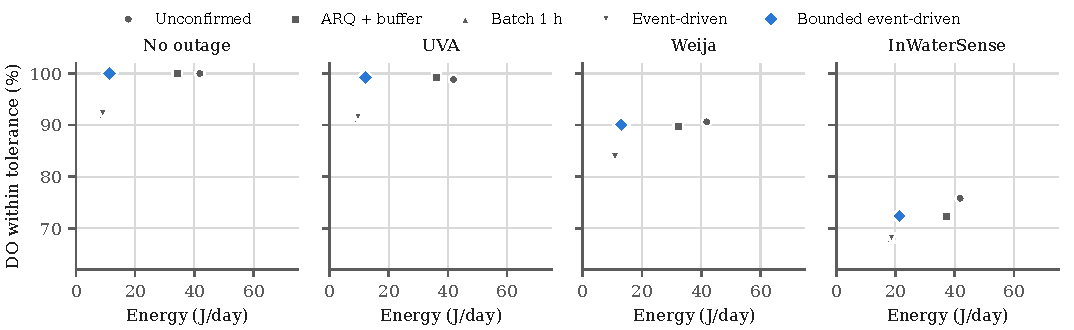
\includegraphics[width=\textwidth]{fig_tradeoff}
\caption{Held-out year (2024): energy against the real-time picture of DO (share of slots within the L2 tolerance), LoRaWAN SF7, median over sites, one panel per link, all panels on the same vertical scale. Batch~1~h and event-driven batching nearly coincide. The bounded design reaches the picture of per-reading reporting at a fraction of its energy.}
\label{fig:tradeoff}
\end{figure*}

\subsection{Events that start during a gap (H3)}
\label{sec:des-outage}
Table~\ref{tab:onset} and Fig.~\ref{fig:onset} show the detected events whose onset fell in a gap. As expected (H3), every strategy has to wait for the link. Unconfirmed reporting learns of almost none of these events (at most \onsetUnconfKnownMax{} on any link and radio): the alarming readings fall inside the gap and are lost. The buffering strategies learn of at least \onsetBufKnownMin, but only after the gap; the gap, not the reporting scheme, sets this latency. Within it, the immediate alarm probe makes the event-driven designs faster than ARQ + buffer on the water-quality records.

\begin{table}[t]
\centering
\caption{Held-out year (2024): detected events whose onset fell in a gap (LoRaWAN SF7, pooled over sites): number of events, share the server ever learns of, and median latency of those it learns of (hours).}
\label{tab:onset}
\scriptsize
\setlength{\tabcolsep}{2.4pt}
\begin{tabular}{@{}lrrrrrrrr@{}}
\toprule
 & & \multicolumn{3}{c}{Known ever} & \multicolumn{4}{c}{Median latency (h)} \\
\cmidrule(lr){3-5}\cmidrule(l){6-9}
Link & $n$ & Unconf. & ARQ & Event & ARQ & Batch & Event & Bounded \\
\midrule
\tabin{tables/tab_onset.tex}
\bottomrule
\end{tabular}
\end{table}

\begin{figure*}[t]
\centering
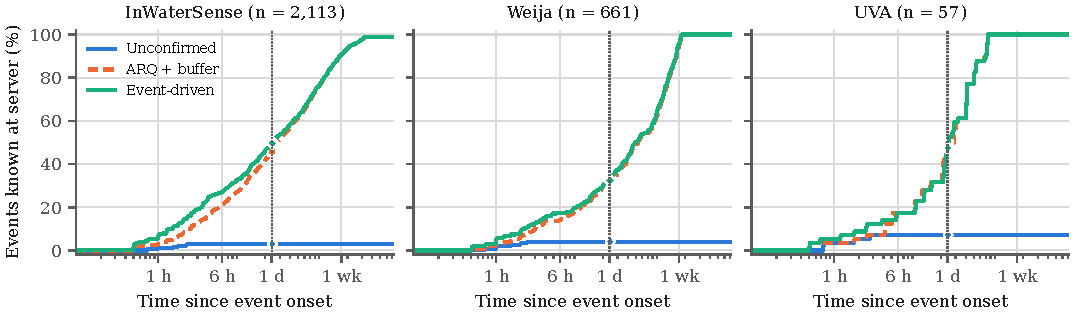
\includegraphics[width=\textwidth]{fig_outage_onset}
\caption{Held-out year (2024): detected events whose onset fell in a gap, share known at the server by the time on the horizontal axis (LoRaWAN SF7, pooled over sites; markers at 1~day). Unconfirmed reporting learns of almost none; the buffering strategies learn of nearly all, after the gap.}
\label{fig:onset}
\end{figure*}

\subsection{Packing order and tolerance level (H8--H10)}
\label{sec:des-sens}
On SF12 a frame holds only \rpfSfTwelve{} readings, so an hourly batch at 15-min sampling needs two frames, and the duty cycle delays the second. With first-in-first-out packing the newest reading rode in the second frame, and in the first development run the server's picture on the no-outage link fell to \fifoMinSfTwelve{} at worst instead of 100\%. H8 predicted that packing the newest reading first would make it exact everywhere. As written, H8 failed: the picture fell short at one site (\hEightPreSite, 5-min sampling, SF12), with a minimum of \hEightPreMin{}. The cause was two implementation defects, each a departure from the stated design: the reading promoted to the first frame could be a placeholder for a sensor gap rather than the newest valid reading, and the node's copy of the server counted readings as known as soon as their upload began, although at 5-min sampling an SF12 upload spans several slots. Both were fixed (D4); the lesson is general: a node that mirrors its server must model when data arrive, not only whether. With the fix, newest-first packing is within tolerance at every scored slot of the no-outage link, on every site, parameter and radio, in both years, at \nfRatioMin--\nfRatioMax{} times the energy of first-in-first-out packing (2024).

The tolerance level sets the price of the bound (Table~\ref{tab:sensitivity}). The picture stays within 1 percentage point of per-reading reporting at every level (H9), and per-reading ARQ uses \levOneArqOverMinConf--\levOneArqOverMaxConf{} the bounded design's energy at L1, \levTwoArqOverMinConf--\levTwoArqOverMaxConf{} at L2 and \levThreeArqOverMinConf--\levThreeArqOverMaxConf{} at L3 (H10).

\begin{table}[t]
\centering
\caption{Held-out year (2024): energy (median J/day over sites, LoRaWAN SF7, series without injected events) at three tolerance levels, the median over sites of each site's ARQ / Bounded energy ratio, and the lowest within-tolerance share over the four parameters (median site). ARQ: ARQ + buffer.}
\label{tab:sensitivity}
\scriptsize
\setlength{\tabcolsep}{2.5pt}
\begin{tabular}{@{}llrrrrr@{}}
\toprule
 & & \multicolumn{2}{c}{Energy (J/day)} & & \multicolumn{2}{c}{Within tolerance} \\
\cmidrule(lr){3-4}\cmidrule(l){6-7}
Level & Link & ARQ & Bounded & ARQ/Bounded & Bounded & ARQ \\
\midrule
\tabin{tables/tab_sensitivity.tex}
\bottomrule
\end{tabular}
\end{table}

\subsection{Where the server's state comes from}
\label{sec:des-ack}
On LoRaWAN, the evaluation above takes a confirmed uplink's acknowledgement, which comes from the network server, as proof that the application server shows the reading. If the node may not assume this, it keeps the bound for both possible server states until an application acknowledgement returns in the downlink of a later uplink (Sec.~\ref{sec:des-design}). On the development sites, this costs \ackCostMin{} to \ackCostMax{} more energy than trusting the network server, because the node uploads again whenever the older state could be out of tolerance; the picture of the median site stays within \ackPicWorst{} percentage points of per-reading reporting, and per-reading ARQ still uses \ackArqOverMin--\ackArqOverMax{} as much energy. On NB-IoT the question does not arise: its confirmation is the application's reply.

The answer to RQ4 is yes, with the link up, and on data not used to design the scheme. Bounded event-driven batching delivers every reading the node generates, raises alarms as fast as per-reading reporting, keeps the server's picture within a chosen tolerance as often as per-reading reporting does, and costs \boundedOverBatchMinConf--\boundedOverBatchMaxConf{} the energy of plain hourly batching, while per-reading ARQ uses \arqOverBoundedMinConf--\arqOverBoundedMaxConf{} as much energy on the held-out year. What no scheme can fix is the gap itself: events and data during a gap reach the server only when the link returns.
